%%%%%%%%%%%%%%%%%%%%%%%%%%%%%%%%%%%%%%%%%
% Short Sectioned Assignment LaTeX Template Version 1.0 (5/5/12)
% This template has been downloaded from: http://www.LaTeXTemplates.com
% Original author:  Frits Wenneker (http://www.howtotex.com)
% License: CC BY-NC-SA 3.0 (http://creativecommons.org/licenses/by-nc-sa/3.0/)
%%%%%%%%%%%%%%%%%%%%%%%%%%%%%%%%%%%%%%%%%

%----------------------------------------------------------------------------------------
%	PACKAGES AND OTHER DOCUMENT CONFIGURATIONS
%----------------------------------------------------------------------------------------

\documentclass[paper=a4, fontsize=11pt]{scrartcl} % A4 paper and 11pt font size

% ---- Entrada y salida de texto -----

\usepackage[T1]{fontenc} % Use 8-bit encoding that has 256 glyphs
\usepackage[utf8]{inputenc}
\usepackage{fourier} % Use the Adobe Utopia font for the document - comment this line to return to the LaTeX default

% ---- Idioma --------

\usepackage[spanish, es-tabla]{babel} % Selecciona el español para palabras introducidas automáticamente, p.ej. "septiembre" en la fecha y especifica que se use la palabra Tabla en vez de Cuadro

% ---- Otros paquetes ----

\usepackage{url} % ,href} %para incluir URLs e hipervínculos dentro del texto (aunque hay que instalar href)
\usepackage{amsmath,amsfonts,amsthm} % Math packages
%\usepackage{graphics,graphicx, floatrow} %para incluir imágenes y notas en las imágenes
\usepackage{graphics,graphicx, float} %para incluir imágenes y colocarlas
\usepackage{epstopdf}
\usepackage[gen]{eurosym} %para incluir el símbolo del euro
\usepackage{cite} %para incluir citas del archivo <nombre>.bib
%\graphicspath{/images}

% Para hacer tablas comlejas
%\usepackage{multirow}
%\usepackage{threeparttable}

%\usepackage{sectsty} % Allows customizing section commands
%\allsectionsfont{\centering \normalfont\scshape} % Make all sections centered, the default font and small caps

\usepackage{fancyhdr} % Custom headers and footers
\pagestyle{fancyplain} % Makes all pages in the document conform to the custom headers and footers
\fancyhead{} % No page header - if you want one, create it in the same way as the footers below
\fancyfoot[L]{} % Empty left footer
\fancyfoot[C]{} % Empty center footer
\fancyfoot[R]{\thepage} % Page numbering for right footer
\renewcommand{\headrulewidth}{0pt} % Remove header underlines
\renewcommand{\footrulewidth}{0pt} % Remove footer underlines
\setlength{\headheight}{13.6pt} % Customize the height of the header

\numberwithin{equation}{section} % Number equations within sections (i.e. 1.1, 1.2, 2.1, 2.2 instead of 1, 2, 3, 4)
\numberwithin{figure}{section} % Number figures within sections (i.e. 1.1, 1.2, 2.1, 2.2 instead of 1, 2, 3, 4)
\numberwithin{table}{section} % Number tables within sections (i.e. 1.1, 1.2, 2.1, 2.2 instead of 1, 2, 3, 4)

\setlength\parindent{0pt} % Removes all indentation from paragraphs - comment this line for an assignment with lots of text

\newcommand{\horrule}[1]{\rule{\linewidth}{#1}} % Create horizontal rule command with 1 argument of height


%----------------------------------------------------------------------------------------
%	TÍTULO Y DATOS DEL ALUMNO
%----------------------------------------------------------------------------------------

\title{
\normalfont \normalsize
\textsc{\textbf{Ingeniería de Servidores (2016-2017)} \\ Grado en Ingeniería Informática \\ Universidad de Granada} \\ [25pt] % Your university, school and/or department name(s)
\horrule{0.5pt} \\[0.4cm] % Thin top horizontal rule
\huge Memoria Práctica 2 \\ % The assignment title
\horrule{2pt} \\[0.5cm] % Thick bottom horizontal rule
}

\author{Adrián Morente Gabaldón} % Nombre y apellidos

\date{\normalsize\today} % Incluye la fecha actual

%----------------------------------------------------------------------------------------
% DOCUMENTO
%----------------------------------------------------------------------------------------

\begin{document}

\maketitle % Muestra el Título

\newpage %inserta un salto de página

\tableofcontents % para generar el índice de contenidos

\listoffigures

\listoftables

\newpage


\section{a) Liste los argumentos de yum necesarios para instalar, buscar y eliminar
paquetes. b) ¿Qué ha de hacer para que yum pueda tener acceso a Internet en el PC
del aula? (Pistas: archivo de configuración en /etc, proxy: stargate.ugr.es:3128)
c) ¿Cómo añadimos un nuevo repositorio?}

	\subsection{Argumentos para uso de yum}
	Los argumentos necesarios para el uso de yum para instalación, búsqueda y eliminación de paquetes son, respectivamente, los siguientes \cite{yum-admin}:
	\begin{itemize}
		\item sudo yum \emph{install} -y <nombre>
		\item sudo yum \emph{search} <nombre>
		\item sudo yum \emph{remove} <nombre>
	\end{itemize}

	\subsection{Acceso a Internet en el PC del aula}
	Como vemos en la documentación de CentOS \cite{yum-proxy}, para utilizar yum con una conexión a Internet mediante proxy, hemos de modificar el archivo de configuración ubicado en \emph{/etc/yum.conf} cumplimentando el siguiente contenido: 
	\begin{verbatim}
	# The proxy server - URL completa del proxy y número del puerto TCP
	proxy = http://stargate.ugr.es:3128
	# Detalles de la cuenta de usuario
	proxy_username = <usuario>
	proxy_password = <contraseña>
	\end{verbatim}	
	
	\subsection{Añadir repositorios a yum}
	Los repositorios son el modo de almacenamiento de todas las fuentes y enlaces de donde podemos obtener los paquetes disponibles para su instalación en el sistema. Para añadir repositorios a yum disponemos de varias opciones, las cuales se mantienen todas por temas de retrocompatibilidad con versiones más antiguas del sistema operativo. Esta vez, usaremos la documentación oficial de RedHat para ilustrarnos \cite{yum-repo} ya que como sabemos, el código que compone CentOS deriva (gracias a su comunidad) del proyecto RedHat; y que por tanto nos es muy útil en cuanto al aprendizaje de Yum.
	\begin{itemize}
		\item En el archivo ubicado en /etc/yum.repos.d hemos de añadir un fichero de texto con extensión \emph{.repo}, cuyo contenido sea la URL del repositorio deseado. A continuación, actualizamos la lista en caché de yum (con \emph{sudo yum update}) y ya lo tenemos a nuestra disposición para su uso.
		\item La otra opción y más rápida, es ejecutar como usuario el comando \emph{sudo yum-config-manager --add-repo <URL>}.
	\end{itemize}


\section{a) Liste los argumentos de APT necesarios para instalar, buscar y eliminar
paquetes. b) ¿Qué ha de hacer para que APT pueda tener acceso a Internet en el PC
del aula? c) ¿Cómo añadimos un nuevo repositorio?}

	\subsection{Argumentos para uso de APT}
	Los argumentos necesarios para el uso de APT para instalación, búsqueda y eliminación de paquetes son, respectivamente, los siguientes:
	\begin{itemize}
		\item sudo \emph{apt-get install} -y <nombre>
		\item sudo \emph{apt-cache search} <nombre>
		\item sudo \emph{apt-get remove} <nombre>
	\end{itemize}

	\subsection{Acceso a Internet en el PC del aula}
	A diferencia de CentOS, en Ubuntu Server es más sencillo utilizar una proxy para poder conectarnos a Internet a través del PC del aula; tan solo hay que introducir y ejecutar el siguiente comando en la terminal:
	\begin{verbatim}
	export HTTP_PROXY=http://stargate.ugr.es:3128
	\end{verbatim}
	
	\subsection{Añadir repositorios a APT}
	Para añadir repositorios a la herramienta APT, tenemos varias alternativas bien conocidas:
	\begin{itemize}
		\item El comando \emph{sudo add-apt-repository ppa:<nombre-repositorio>} es la forma más rápida de incluir un repositorio; acto que debemos seguir con el comando \emph{sudo apt-get update} para actualizar la caché de repositorios de APT y poder empezar a utilizarlos.
		\item Otra forma es introducir la URL del repositorio deseado en el archivo de configuración de APT \emph{/etc/apt/sources.list}; cosa que podemos hacer tanto a través de un editor de textos, o con el siguiente comando en la terminal:
		\begin{verbatim}
			<url> >> /etc/apt/sources.list
		\end{verbatim} 
	\end{itemize}
	

\section{a) ¿Con qué comando puede abrir/cerrar un puerto usando ufw? Muestre un ejemplo de cómo lo ha hecho. b) ¿Con qué comando puede abrir/cerrar un puerto usando firewall-cmd en CentOS? Muestre un ejemplo de cómo lo ha hecho. c) Utilice el comando nmap para ver que, efectivamente, los puertos están accesibles.}

	\subsection{Comandos de apertura/cerrado de puertos con ufw}
	Como vemos fácilmente en el manual de ufw a través de la terminal en Ubuntu, podemos abrir y cerrar puertos con el comando \emph{sudo ufw enable/disable}. Para la muestra, he realizado el cerrado y la consiguiente reapertura de los puertos 22 y 80; que se corresponden con los servicios \emph{SSH} y \emph{http} respectivamente.
	Otra forma de aceptar el acceso al servicio proporcionado por un puerto, es utilizar \emph{ufw allow/reject <número>[/protocolo]}; de forma que podemos aceptar (o denegar con \emph{reject}) las solicitudes al puerto identificado por \emph{<número>} además de poder proporcionar el tipo de protocolo deseado (TCP o UDP). Si no especificamos este último parámetro, se aceptarán/denegarán las solicitudes de ambos tipos. Esto se documenta en la siguiente imagen:
	\begin{figure}[H]
		\centering
		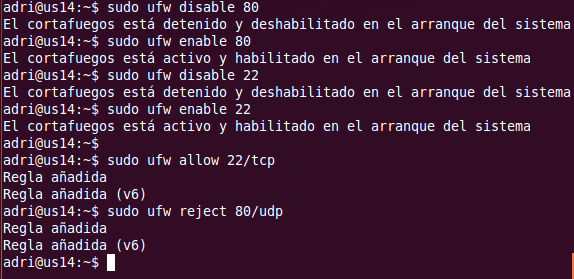
\includegraphics[scale=0.75]{ufw-enable}
		\caption{Cierre y reapertura de puertos para SSH y HTTP. - Adrián Morente Gabaldón [20/11/2016]}
		\label{fig:figura1}
	\end{figure}

	\subsection{Comandos de apertura/cerrado de puertos con firewall-cmd}
	Mientras que en Ubuntu hemos utilizado \emph{ufw} para la administración de puertos, en CentOS utilizamos la herramienta \emph{firewall-cmd}, cuya funcionalidad viene bien explicada en su propio manual, y de cuyas opciones más destacadas hice uso en la prueba adjunta más abajo.
	Para empezar, comprobamos que el firewall del sistema está activo y en ejecución con el comando \emph{systemctl status firewalld}. En caso de que no lo esté, lo activamos fácilmente con \emph{systemctl enable firewalld}.
	Aunque en su documentación muestran muchos usos y comandos distintos, nos restringiremos por ahora a listar los puertos abiertos, y abrir o cerrar algunos; todo esto mediante las siguientes opciones de \emph{firewall-cmd}:
	\begin{itemize}
		\item \textbf{firewall-cmd \emph{--list-ports}}: imprime en pantalla los puertos que hemos abierto manualmente.
		\item \textbf{firewall-cmd \emph{--add-port=<número>/<protocolo>}}: añade a firewalld (o abre, más bien) el puerto especificado, aceptando las solicitudes que incluyen el protocolo determinado. (Similar a lo mencionado previamente con \emph{ufw} en Ubuntu Server).
		\item \textbf{firewall-cmd \emph{--remove-port=<número>/<protocolo>}}: elimina de firewalld (o cierra) el puerto especificado para un protocolo dado. Comportamiento similar pero contrario al punto anterior.
	\end{itemize}
	\begin{figure}[H]
		\centering
		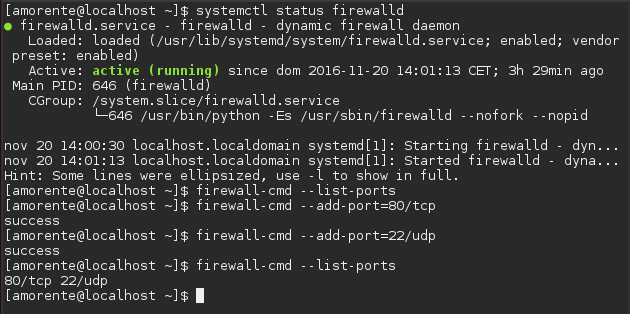
\includegraphics[scale=0.6]{firewall-ports}
		\caption{Apertura de puertos, con sus correspondientes comprobaciones. - Adrián Morente Gabaldón [20/11/2016]}
		\label{fig:figura2}
	\end{figure}

	\subsection{Uso de nmap para listar puertos abiertos}
	Otra forma de comprobar qué servicios estamos ofreciendo de forma activa es mediante el uso de la herramienta \emph{nmap}. Mientras que en Ubuntu Server viene instalada por defecto, en mi caso he tenido que instalarla manualmente en CentOS. Procederemos de la siguiente forma:
	\begin{verbatim}
	nmap localhost
	\end{verbatim}
	Esto listará los servicios disponibles, el estado actual (abierto o cerrado) y el puerto en el que se ofrecen. Como información adicional, muestra la versión de Nmap que estamos utilizando, la fecha y hora actuales, y la latencia de conexión al host entre otras cosas. He aquí una muestra:
	\begin{figure}[H]
		\centering
		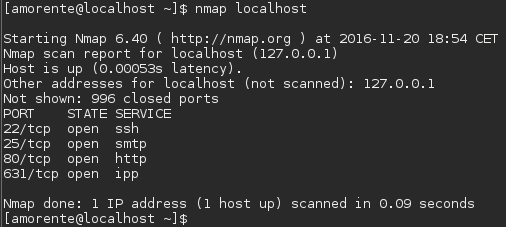
\includegraphics[scale=0.75]{nmap-localhost}
		\caption{Visualización de puertos abiertos del sistema. - Adrián Morente Gabaldón [20/11/2016]}
		\label{fig:figura3}
	\end{figure}
	

\section{¿Qué diferencia hay entre telnet y SSH?}
Tanto telnet como SSH son dos protocolos de red que permiten acceder de forma remota a otra máquina o servidor para facilitar su administración o gestión. La principal diferencia reside en que telnet es una herramienta más antigua, quizás ya en desuso debido a SSH, que viene a implementar la misma funcionalidad pero de una manera más segura y efectiva. \emph{Secure Shell}, que se trata del significado de las siglas de SSH, viene reemplazando a telnet en prácticamente cualquier lugar, y es la herramienta de gestión remota más usada hoy día.
\begin{itemize}
	\item Mientras que telnet envía los datos en texto plano, SSH utiliza un encriptado para que solo el destinatario reciba el mensaje.
	\item Telnet no utiliza ningún tipo de autenticación, lo que permite acceder al mensaje enviado a cualquiera; mientras que SSH utiliza una clave pública de autenticación que mantiene oculto el envío.
\end{itemize}
Está claro que SSH ofrece una manera más segura de acceder a una máquina remota; la desventaja es que al utilizar un cifrado y una clave pública, se requiere de un mayor ancho de banda para el envío de datos (cosa que hoy en día no notamos, pero que en sus inicios pasó factura con las conexiones lentas).


\section{a) ¿Para qué sirve la opción -X? b) Ejecute remotamente, es decir, desde la máquina anfitriona (si tiene Linux) o desde la otra máquina virtual, el comando gedit en una sesión abierta con SSH. ¿Qué ocurre?}

	\subsection{Opción -X de SSH}
	Como vemos en el manual oficial de SSH (ya sea a través de consola o desde la web de OpenSSH \cite{ssh-man}), la opción -X nos permite la ejecución con entorno gráfico de programas en la máquina remota pero en el núcleo del cliente. Es decir, la máquina servidor tan solo envía el núcleo del programa pero la interfaz gráfica se ejecuta en el entorno del cliente cargada de forma local. Esto supone una gran ventaja ya que libera mucha carga de envío de datos a través de la red.
		
	\subsection{Ejecución remota con interfaz gráfica mediante SSH}
	Ya hemos visto el uso de \emph{ssh -X} en el punto anterior, y ahora pasaremos a un caso práctico. 
	\begin{enumerate}[1.]
		\item Para empezar, tenemos las dos máquinas virtuales de CentOS 7 y Ubuntu Server 14.04 encendidas, ambas con la terminal abierta.
		\item A partir del comando \emph{ifconfig} en ambas máquinas, la terminal nos muestra las redes a las que están conectadas cada una de las máquinas, con sus correspondientes direcciones.
		\item Una vez que tenemos las direcciones (eth0 en Ubuntu Server y enp0s3 en CentOS, en mi caso), probamos a hacer ping entre las máquinas, para verificar que existe una vía de comunicación entre ellas.
		\item Hecho esto, pasamos a conectarnos por SSH. Para este supuesto práctico, he probado a conectarme a Ubuntu Server desde CentOS. Para ello, necesitamos ingresar como parámetro a SSH el nombre de usuario con el que queremos iniciar sesión en la máquina remota, junto con la dirección de dicha máquina de la siguiente forma:
		\begin{verbatim}
			ssh -X adri@10.0.2.4
		\end{verbatim}
		\item Hecho esto, SSH nos pedirá la contraseña del usuario especificado y al introducirla correctamente ya tendremos acceso. Llegados aquí, con tan solo ejecutar \emph{gedit} vía SSH ya podremos utilizar dicha herramienta con interfaz gráfica.
	\end{enumerate}
	\begin{figure}[H]
		\centering
		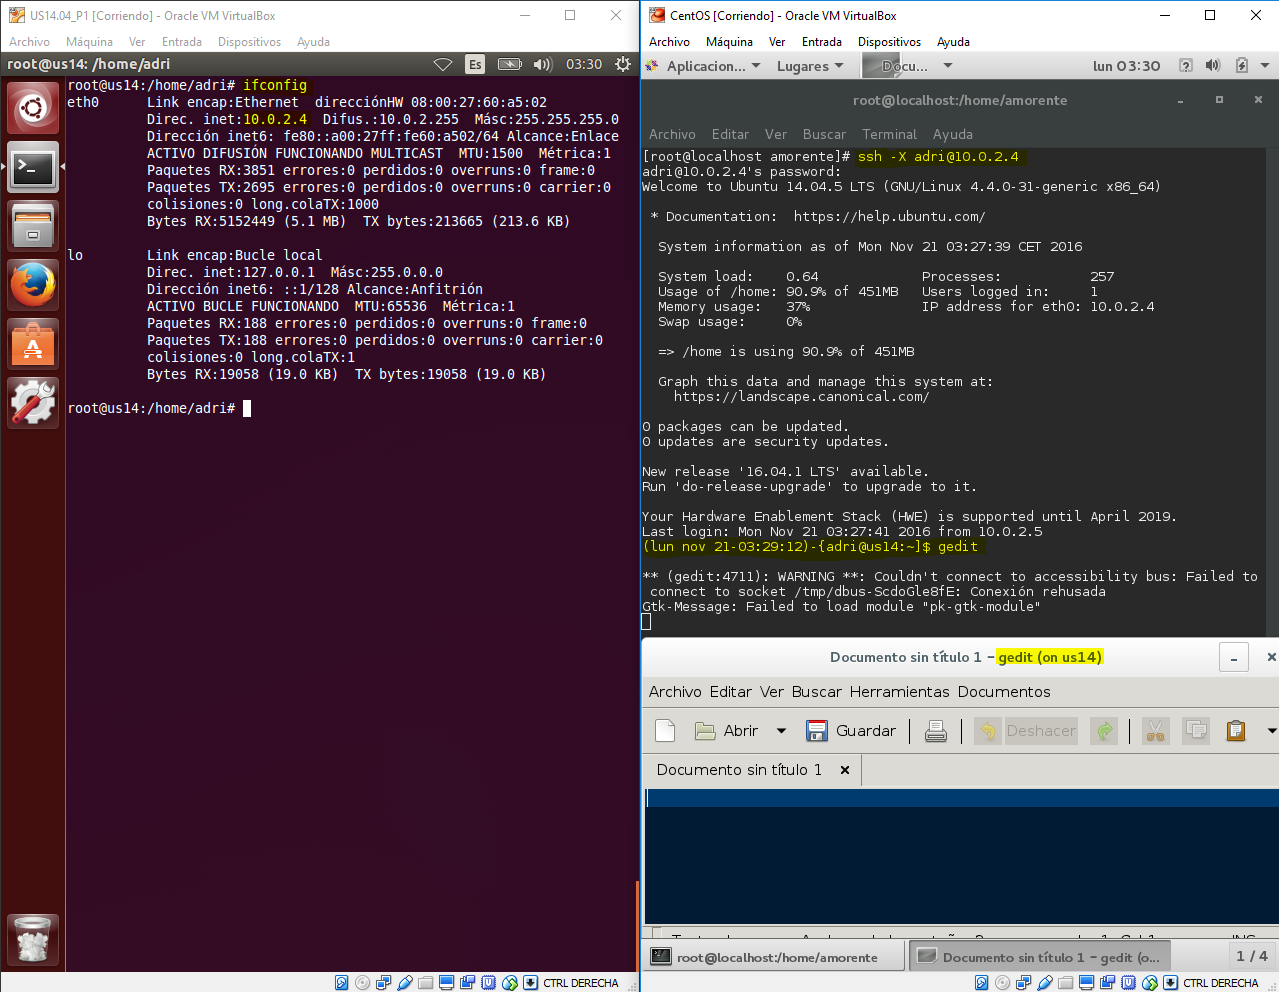
\includegraphics[scale=0.4]{ssh-X}
		\caption{Ejecución de gedit con interfaz gráfica de forma remota a través de SSH. - Adrián Morente Gabaldón [21/11/2016]}
		\label{fig:figura6}
	\end{figure}


\section{Muestre la secuencia de comandos y las modificaciones a los archivos correspondientes para permitir acceder a la consola remota sin introducir la contraseña. Pruebe que funciona. (Pistas: ssh-keygen, ssh-copy-id).}
Si vamos a estar accediendo de forma frecuente a una máquina remota mediante Secure Shell, nos puede interesar saltarnos el paso de introducir la contraseña de usuario cada vez que accedemos. Esto se consigue a través de la importación de una clave pública con el sistema algorítmico \textbf{RSA}, que se trata del algoritmo más utilizado para cifrado y firma digital. El procedimiento a seguir, realizado desde el directorio \emph{/home} del usuario o del administrador raíz, es el siguiente:
\begin{enumerate}[1.]
	\item Para empezar, podemos usar la herramienta \emph{ssh-keygen} para generar una clave dedicada al uso mencionado, y que a través de las opciones \emph{-b} y \emph{-t} nos permite especificar el número de bytes que queremos utilizar en la firma y el algoritmo de cifrado a utilizar, respectivamente.
	\item Tras hacer esto, la herramienta nos preguntará por la ubicación donde deseamos guardar la clave (por defecto se guardará en /home/<usuario>/.ssh/id\_rsa) y la frase de paso con la que queremos proteger dicha clave.
	\item A continuación, usamos el comando \emph{ssh-copy-id} acompañado del nombre de usuario al que deseamos acceder y la dirección IP de la máquina remota. Esto instala la clave pública y la asocia a dicho usuario en dicha máquina.
	\item Para terminar, ya podemos acceder mediante SSH al usuario de la máquina remota sin que nos exija la autenticación correspondiente. Aquí pueden suceder dos cosas:
	\begin{itemize}
		\item Si estamos accediendo como usuario normal sin permisos de administración, al ejecutar la conexión SSH el sistema nos pedirá una vez la frase de paso para desbloquear la clave pública creada anteriormente (que no es lo mismo que introducir la clave del usuario en la máquina remota), y ya accederemos a la máquina deseada.
		\item Si estamos accediendo como usuario \emph{root}, no nos pedirá dicha frase de paso y tendremos acceso directo a la máquina.
	\end{itemize}
\end{enumerate}
\begin{figure}[H]
	\centering
	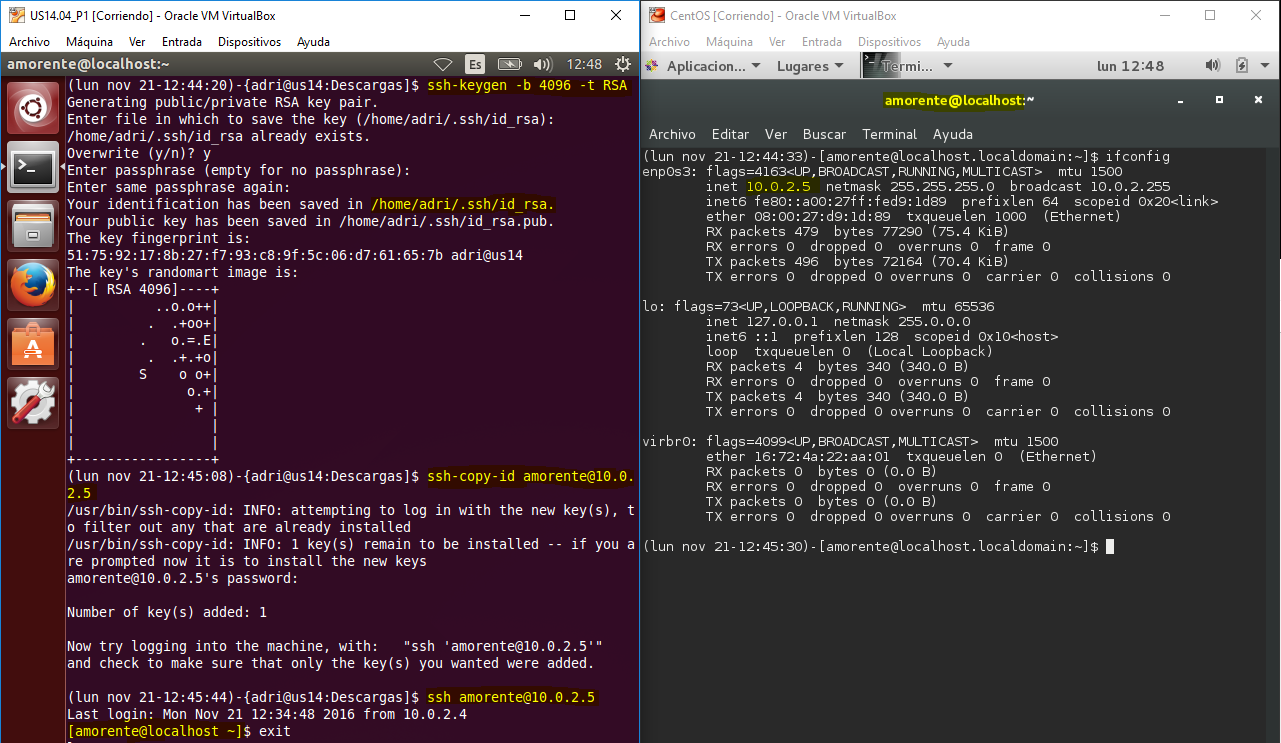
\includegraphics[scale=0.4]{ssh-keygen}
	\caption{Generación de clave privada y acceso de forma remota a través de SSH. - Adrián Morente Gabaldón [21/11/2016]}
	\label{fig:figura7}
\end{figure}


\section{¿Qué archivo es el que contiene la configuración del servicio SSH? ¿Qué parámetro hay que modificar para evitar que el usuario root acceda? Cambie el puerto por defecto y compruebe que puede acceder.}
La configuración del servicio SSH se encuentra en el archivo /etc/ssh/sshd\_config, y obviamente contiene todos los parámetros configurables de dicho servicio. Antes de manipular el fichero de configuración, sería conveniente hacer una copia de seguridad de dicho archivo que pudiéramos restaurar si al configurarlo trastocamos algo que no queríamos y que puede comprometer a la estabilidad o el funcionamiento del sistema. Una vez hecho esto, pasamos a la configuración.
\begin{itemize}
	\item Para evitar que pueda acceder el usuario root, buscaremos dentro de dicho archivo el apartado de \emph{Autenticación} (\emph{Authentication}, como lo veremos en inglés); y encontramos que el segundo parámetro dentro de éste es \emph{PermitRootLogin} con el atributo puesto a \emph{no}. Lo que tenemos que hacer es simplemente descomentar esta línea para que pase a ser efectiva.
	\begin{verbatim}
		#PermitRootLogin no
	\end{verbatim}
	\item Para cambiar el puerto por defecto nos iremos a modificar la primera línea de configuración del archivo, justo debajo de los comentarios de introducción. Encontramos la siguiente línea, que solo tenemos que descomentar y cambiar el número de puerto al que nosotros queramos (pero con un valor mayor a 1024, ya que por debajo de este número, todos los puertos están restringidos):
	\begin{verbatim}
		#Port 22
	\end{verbatim}
\end{itemize}
Cabe destacar que siempre que hagamos alguna de estas modificaciones, tendremos que reiniciar el servicio como vimos en ejercicios anteriores para que dicha modificación entre en vigor. Para este caso práctico, he cambiado el puerto de acceso a SSH en CentOS por el 2222, he añadido dicho puerto al firewall y he reiniciado el servicio (con \emph{systemctl restart sshd.service} en modo root). Además, según vemos en el inicio del archivo \emph{sshd\_config}, en CentOS (y sistemas SELinux) necesitaremos ejecutar el siguiente comando para que el servicio acepte otro puerto:
\begin{verbatim}
	semanage port -a -t ssh_port_t -p tcp 2222
\end{verbatim}
Dicho comando hará que el servicio SSH acepte solicitudes con el protocolo TCP a través del puerto 2222. En la prueba práctica, aparece un error al ejecutarlo porque ya lo definí antes, pero tuve que volver a hacerlo para poder tomar la captura. Acto seguido vemos que funciona:
\begin{figure}[H]
	\centering
	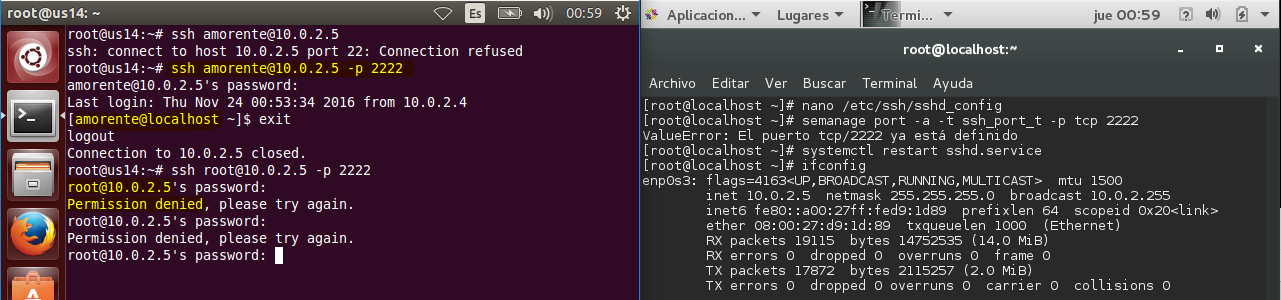
\includegraphics[scale=0.4]{ssh-port}
	\caption{Acceso correcto con usuario normal, pero acceso de forma errónea como usuario root. - Adrián Morente Gabaldón [23/11/2016]}
	\label{fig:figura21}
\end{figure}


\section{Indique si es necesario reiniciar el servicio ¿Cómo se reinicia un servicio en Ubuntu? ¿y en CentOS? Muestre la secuencia de comandos para hacerlo.}
Sí, es necesario reiniciar los servicios al hacer una modificación de este tipo, tanto en Ubuntu Server como en CentOS. En ambos sistemas operativos habremos de tener permisos de administración para ello. Realizamos tal tarea en cada uno de los sistemas operativos con los siguientes comandos:
\begin{itemize}
	\item \textbf{Reiniciar un servicio en Ubuntu}: es fácil de hacer utilizando simplemente el comando \emph{sudo service restart <nombre-servicio>}. Acto seguido, la terminal nos imprime un mensaje confirmando si se ha realizado la acción deseada o no. En la imagen adjunta también utilizo otras utilidades como \emph{stop} y \emph{start} para mostrar cómo detener e iniciar los servicios; (en este caso, SSH y MySQL):
	- Para un caso práctico más ilustrativo, reinicio los servicios \emph{mysql} y \emph{SSH}, viendo en todo momento el estado actual gracias al mensaje devuelto por la terminal. Acto seguido, a modo de prueba, detengo \emph{SSH} manualmente con \emph{stop} y lo vuelvo a iniciar con \emph{start}. 
	\begin{figure}[H]
		\centering
		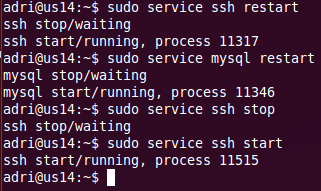
\includegraphics[scale=0.75]{service-ubuntu}
		\caption{Reinicio de servicios en Ubuntu Server. - Adrián Morente Gabaldón [20/11/2016]}
		\label{fig:figura4}
	\end{figure}
	- Para un caso ilustrativo, detenemos el servicio de HTTP e imprimimos su estado, que como vemos es \textbf{dead}. A continuación, mediante la orden vista previamente, reiniciamos el servicio y volvemos a imprimir su estado, siendo \textbf{running} esta vez.
	\item \textbf{Reiniciar un servicio en CentOS}: en CentOS también es sencillo manipular servicios, cosa que hacemos mediante el uso de \emph{systemctl} con las diversas opciones que podemos consultar en su propio manual a través de la terminal. En el supuesto práctico, utilizo la opción \emph{stop} para detener el servicio de ejemplo, muestro su estado con \emph{status}, lo reinicio con la opción \emph{restart} y vuelvo a monitorizar su estado.
	\begin{figure}[H]
		\centering
		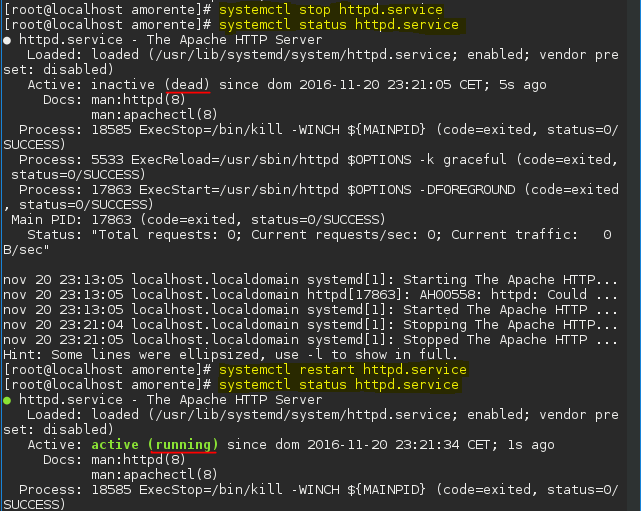
\includegraphics[scale=0.75]{systemctl-centos}
		\caption{Reinicio de servicios en CentOS. - Adrián Morente Gabaldón [22/11/2016]}
		\label{fig:figura5}
	\end{figure}
\end{itemize}


\section{Muestre los comandos que ha utilizado en Ubuntu Server y en CentOS (aunque en este último puede utilizar la GUI, en tal caso, realice capturas de pantalla). Compruebe que la instalación ha sido correcta.}
Tanto en Ubuntu como en CentOS utilizaremos la terminal para la instalación de LAMP, ya que el proceso es sencillo y más liviano de este modo.
\begin{itemize}
	\item En Ubuntu Server, con una sola línea conseguiremos instalar a la vez \emph{Apache2} para servir HTTP, \emph{MySQL} para la gestión de nuestra base de datos y \emph{PHP} para la administración de la(s) página(s) web que vayamos a ofrecer. Para ello, utilizamos el siguiente comando (con APT):
	\begin{verbatim}
		sudo apt-get install lamp-server^
	\end{verbatim}
	\item Por otro lado, en CentOS necesitaremos introducir tres líneas en la terminal para que YUM instale todos los paquetes necesarios (similares a los del punto anterior en Ubuntu Server). El primero instalará el servicio \emph{Apache2}, el segundo instalará \emph{PHP} y el último \emph{MariaDB} para la comunicación con nuestra base de datos:
	\begin{verbatim}
		sudo yum install httpd
		sudo yum install php
		sudo yum install mariadb-server
	\end{verbatim}
\end{itemize}
Para finalizar, vemos dos capturas de pantalla mostrando que el servidor web ya está instalado en ambos sistemas operativos.
Accediendo a la dirección \emph{localhost} desde el navegador de Ubuntu Server llegamos a esta página. Si leemos el mensaje aportado, comprobamos que Apache2 está correctamente instalado y listo para actuar a modo de servidor web. Para ofrecer una página web distinta a la del ejemplo, tendremos que incluir nuestro \emph{index.html} modificado en el directorio \emph{/var/www/html} del que Apache2 toma los datos:
\begin{figure}[H]
	\centering
	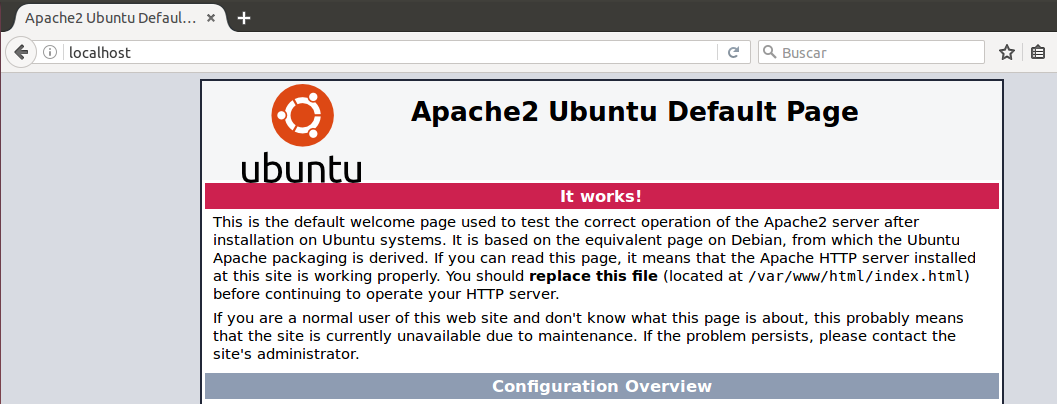
\includegraphics[scale=0.5]{apache-ubuntu}
	\caption{Comprobación de la instalación del servicio Apache en Ubuntu Server. - Adrián Morente Gabaldón [22/11/2016]}
	\label{fig:figura8}
\end{figure}
Accediendo a la dirección \emph{localhost} desde el navegador de CentOS llegamos a esta página. Si leemos el mensaje aportado, comprobamos que Apache está correctamente instalado y listo para actuar a modo de servidor web. Esta es la apariencia que tiene una página web impulsada por Apache y CentOS; por lo que si llegamos a verla se debe a que o no hemos definido ya una página web, o está experimentando problemas (como informa la misma página). Para ofrecer una página web distinta habremos de incluir nuestro \emph{index.html} modificado en el directorio \emph{/var/www/html} del que Apache toma los datos:
\begin{figure}[H]
	\centering
	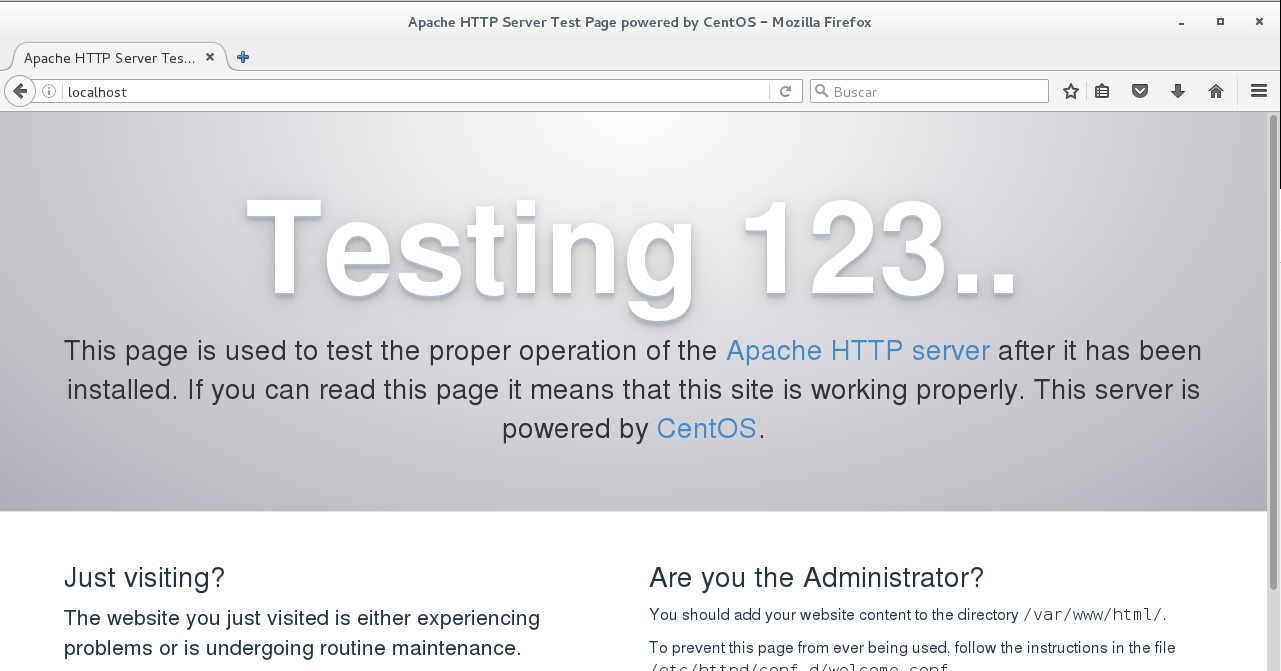
\includegraphics[scale=0.45]{apache-centos}
	\caption{Comprobación de la instalación del servicio Apache en CentOS. - Adrián Morente Gabaldón [22/11/2016]}
	\label{fig:figura9}
\end{figure}


\section{Realice la instalación usando GUI o PowerShell y compruebe que el servicio está funcionando accediendo a la MV a través de la anfitriona.}
Como cualquier instalación de un programa o servicio en Windows, instalar IIS es extremadamente sencillo; tan solo hay que entrar a la configuración inicial del servidor Windows y elegir la función \emph{Agregar roles}. De entre las opciones sugeridas, elegiremos la de IIS junto con todas las características pedidas en el guión de esta práctica.

Una vez que hemos añadido todo lo deseado, apagaremos la máquina, de forma que en VirtualBox podamos añadir un segundo adaptador de red con conexión \emph{Host-Only}. Esto lo hacemos para poder acceder a las direcciones IP de la máquina virtual desde nuestra máquina anfitriona (que en mi caso está corriendo con Windows 10, para un uso más sencillo y estable de la virtualización).

Para comprobar de forma veraz que IIS está funcionando en Windows Server, comenzamos por obtener su dirección IP a través de PowerShell con el comando \emph{ipconfig}. A continuación, introducimos dicha dirección IP en el navegador de la máquina anfitriona; el cual nos mostrará la siguiente página de demostración de IIS:
\begin{figure}[H]
	\centering
	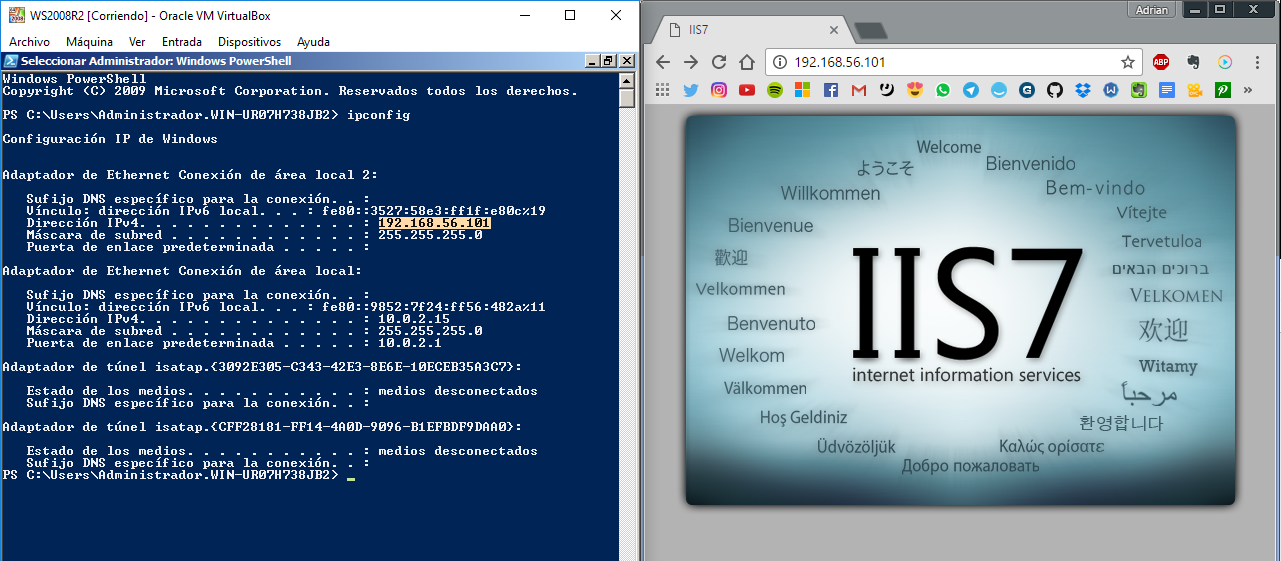
\includegraphics[scale=0.47]{iis-windows}
	\caption{Página de demostración del servicio IIS. - Adrián Morente Gabaldón [22/11/2016]}
	\label{fig:figura10}
\end{figure}


\section{Muestre un ejemplo de uso del comando patch (p.ej. un programas sencillo HolaMundo con algún fallo concreto [bucle infinito, por ejemplo], y otro programa con dicho fallo arreglado)}
El comando patch se utiliza para corregir fallos o aplicar pequeñas modificaciones a un código de alto nivel a partir de un archivo \emph{diff} que incluye dichas modificaciones a realizar. El procedimiento es sencillo, y se basa en:
\begin{itemize}
	\item Comparar con \emph{diff} dos archivos (uno de ellos el que deseamos corregir, y otro con los errores corregidos), redirigiendo el resultado de la operación a un archivo con extensión \emph{.patch}. Este archivo contendrá las diferencias encontradas entre los dos ficheros.
	\item Ejecutar el comando \emph{patch} con dos argumentos: uno el archivo pendiente de modificar, y por último el archivo con extensión \emph{.patch} creado en el paso anterior. Esto aplicará el parche al fichero.
	\item Para terminar, si estamos trabajando con un lenguaje de programación compilado como C o C++, habremos de recompilar el código arreglado. Si se trata de un lenguaje interpretado como Ruby o Python podremos ejecutarlo directamente.
\end{itemize} 
Para este caso práctico, he hecho el ejemplo propuesto en clase y mencionado en el enunciado. Tendremos dos archivos de código en C++, y el primero consta del siguiente contenido:
\begin{lstlisting}[language=c]
	#include <iostream>
	using namespace std;
	int main(int argc, char *argv[]){
	  for(int i=0; i<5; i--)
	    cout << "Hola mundo!" << endl;
	  return 0;
	}
\end{lstlisting}
Si nos fijamos un poco, veremos un error en el incremento de la variable interna del bucle for, lo que provoca un bucle infinito. Para solucionar esto, el otro archivo de código tendrá el siguiente contenido:
\begin{lstlisting}[language=c]
	#include <iostream>
	using namespace std;
	int main(int argc, char *argv[]){
	  for(int i=0; i<5; i++)
	    cout << "Hola mundo!" << endl;
	  return 0;
	}
\end{lstlisting}
A continuación, una captura de pantalla con el procedimiento mencionado puesto en práctica. En un principio nos encontramos con el fallo en ejecución (no mostrado aquí ya que es un bucle infinito). Comparamos los archivos en busca de las líneas que, al ser diferentes, sean las que potencialmente están causando el problema. Guardamos las diferencias a aplicar en un archivo \emph{patch} y lo aplicamos al archivo erróneo. Para terminar, recompilamos y ejecutamos el nuevo programa para comprobar su funcionamiento.
\begin{figure}[H]
	\centering
	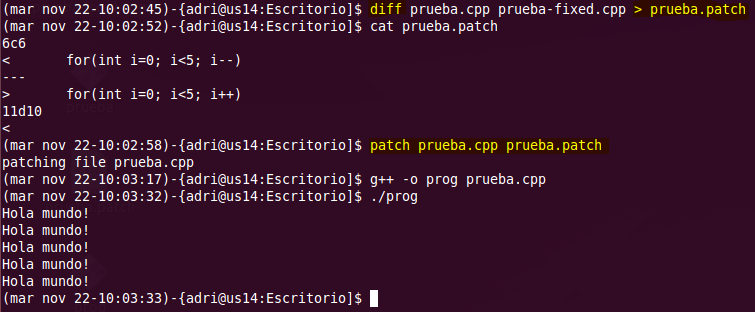
\includegraphics[scale=0.7]{diff-patch}
	\caption{Ejecución de diff-patch con dos programas de prueba. - Adrián Morente Gabaldón [22/11/2016]}
	\label{fig:figura22}
\end{figure}


\section{Realice la instalación de esta aplicación (Webmin) y pruebe a modificar algún parámetro de algún servicio. Muestre las capturas de pantalla pertinentes así como el proceso de instalación.}
Para la instalación de Webmin en Ubuntu Server nos hemos guiado por el manual oficial de su página web \cite{webmin-deb}. Hay dos formas de hacerlo en Ubuntu:
\begin{itemize}
	\item Descargando el archivo completo compilado con extensión \emph{.deb} (el formato admitido por las distribuciones de Linux derivadas de Debian como Ubuntu) e instalándolo ya sea con interfaz gráfica o con el siguiente comando (la X se refiere al número de versión, que podrá variar según cuando descarguemos el archivo y si ha habido actualizaciones):
	\begin{verbatim}
		sudo dpkg -i webmin_X_all.deb
	\end{verbatim}
	\item La otra forma, por la que nos decantaremos, es utilizar el repositorio APT de Webmin. Un aspecto positivo de este método de instalación es que APT resuelve automáticamente las dependencias necesarias, mientras que \emph{dpkg} o el instalador gráfico podrían no hacerlo. El procedimiento para usarlo es:
	\begin{itemize}
		\item Para empezar, añadiremos el repositorio aportado por Webmin al archivo \emph{/etc/apt/sources.list} que, como sabemos, es el archivo de repositorios en los que busca APT los paquetes a instalar. Antes de hacer una modificación directa del archivo, es conveniente hacer una copia de seguridad del archivo por si tocamos algo que no queremos.
		\item A continuación, instalamos la firma GPG del distribuidor de Webmin. Esta es una forma de aportar seguridad a los usuarios que instalan paquetes, ya que reciben un paquete firmado con un nombre propio, que a priori debe ser más seguro que cualquier programa anónimo que encontremos en otro sitio.
		\item Recargamos la caché de repositorios de APT e instalamos el paquete \emph{webmin}.
	\end{itemize}
\end{itemize}
La ejecución práctica de estos pasos previamente detallados es esta:
\begin{lstlisting}[language=bash]
	cp /etc/apt/sources.list /etc/apt/sources.list.bak
	# Webmin APT Repository >> /etc/apt/sources.list
	deb http://download.webmin.com/download/repository sarge contrib 
	    >> /etc/apt/sources.list
	cd /root
	wget http://www.webmin.com/jcameron-key.asc
	apt-key add jcameron-key.asc
	apt-get update
	apt-get install webmin
\end{lstlisting}
Hecho todo esto, abriremos el puerto 10000 en el que trabaja Webmin y nos iremos al navegador a la dirección \emph{https://localhost:10000}. Iniciaremos sesión y llegaremos a la pantalla de demostración de Webmin, en la cula encontramos una completa descripción del sistemaa, ya sea de la fecha actual, las prestaciones de nuestra máquina y el espacio disponible entre otras cosas.
\begin{figure}[H]
	\centering
	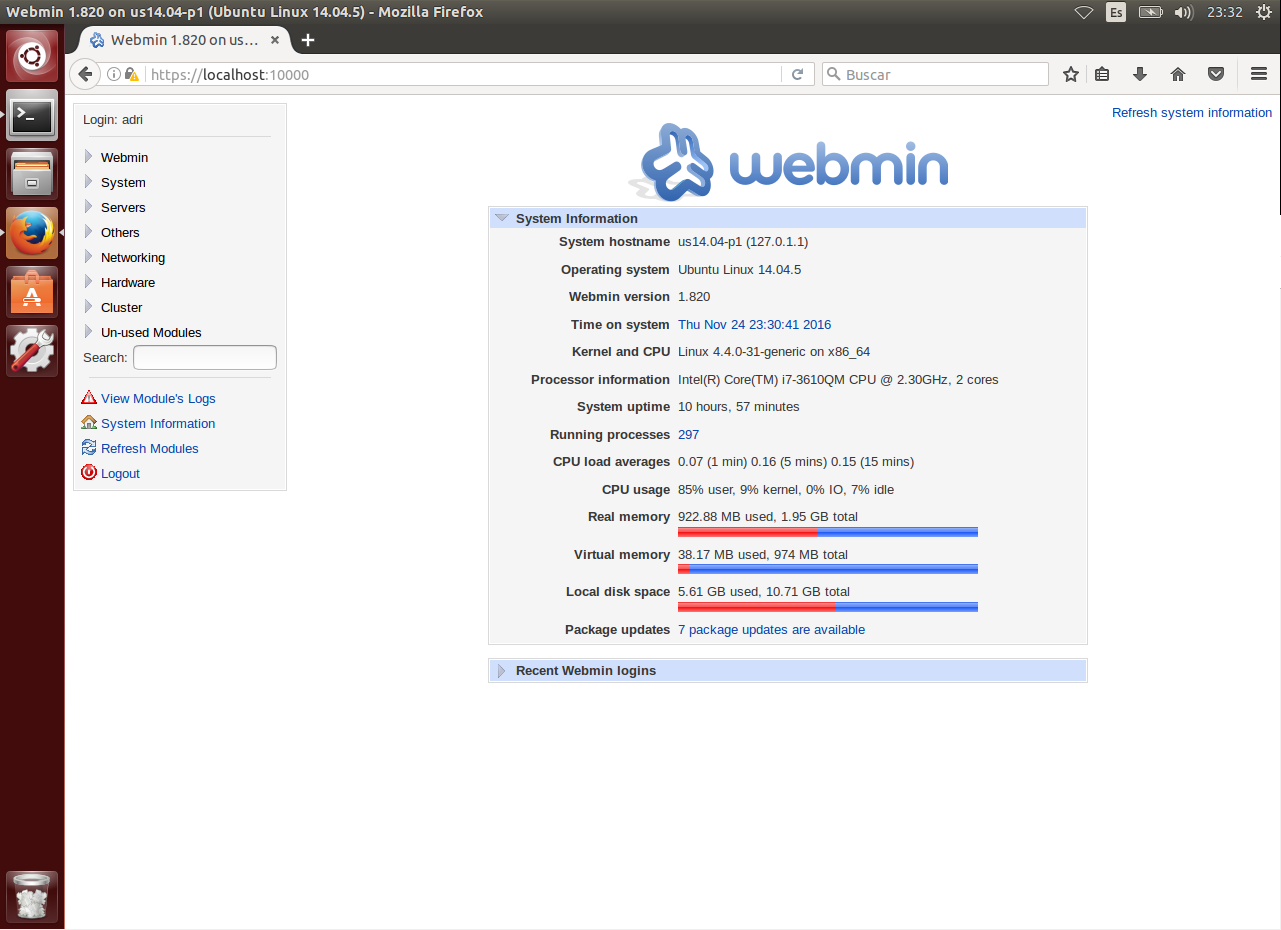
\includegraphics[scale=0.4]{webmin-start}
	\caption{Demostración del funcionamiento de Webmin. - Adrián Morente Gabaldón [24/11/2016]}
	\label{fig:figura17}
\end{figure}
En la columna de la izquierda, Webmin nos propone muchas opciones que podremos configurar. Nos iremos al apartado de Webmin -> Webmin Configuration -> IP Access Control para hacer un ejemplo de configuración. Con la siguiente configuración bloquearíamos el acceso proveniente de direcciones que no figurasen en la lista definida. Es decir, en este caso práctico estaríamos limitando a que solo nuestra máquina de CentOS (con dirección 10.0.2.5 a través de nuestra red NAT) tuviese acceso a nuestra máquina.:
\begin{figure}[H]
	\centering
	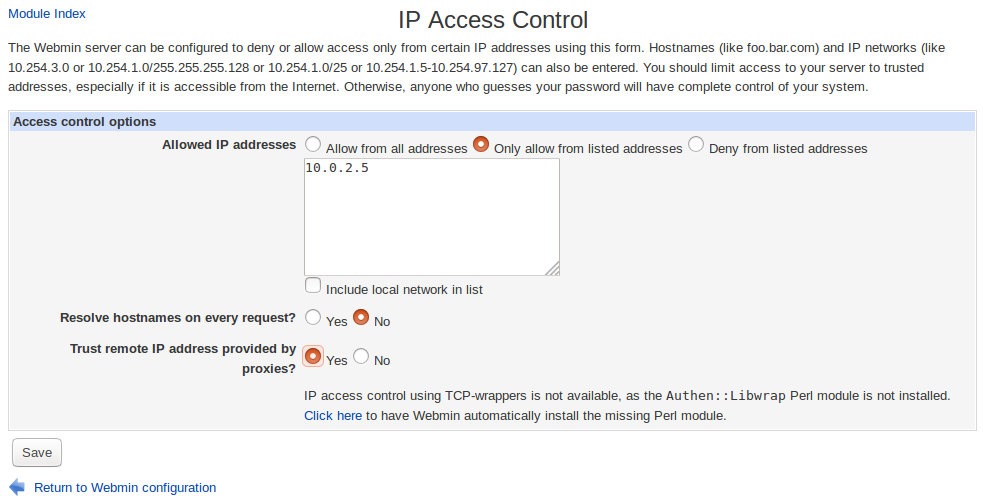
\includegraphics[scale=0.5]{webmin-change}
	\caption{Configuración de bloqueo del acceso al servicio para ciertas direcciones IP. - Adrián Morente Gabaldón [24/11/2016]}
	\label{fig:figura18}
\end{figure}


\section{Instale phpMyAdmin, indique cómo lo ha realizado y muestre algunas capturas de pantalla. Configure PHP para poder importar BDs de hasta 25MiB (en vez de los 8 MiB de límite por defecto). Indique cómo ha realizado el proceso y muestre capturas de pantalla.}
Como vemos en su página oficial \cite{phpmyadmin}, la instalación de phpMyAdmin es fácilmente realizable en Ubuntu (véase la sección de instalación en Debian) con el comando \emph{sudo apt-get install phpmyadmin}. El gestor APT comenzará a descargar y a instalar paquetes, y acto seguido nos mostrará la siguiente imagen:
\begin{figure}[H]
	\centering
	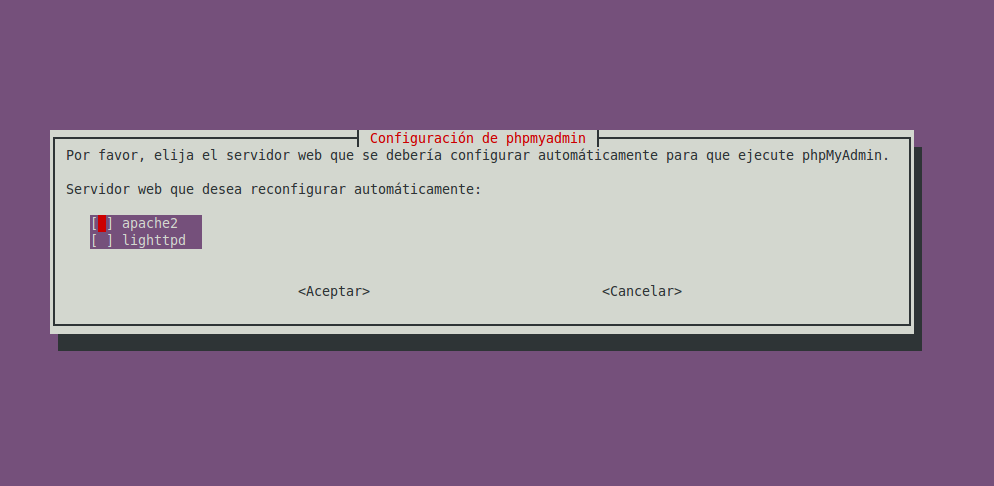
\includegraphics[scale=0.5]{phpmyadmin-apache}
	\caption{Elección de Apache2 para la configuración del servidor web con phpMyAdmin. - Adrián Morente Gabaldón [23/11/2016]}
\end{figure} 
En nuestro caso elegiremos \emph{apache2} (señalándolo y marcándolo con la barra espaciadora), ya que es el servidor web que instalamos antes. A continuación nos pedirá tres contraseñas de protección: una para Apache2, una para la base de datos controlada por MySQL y otra de confirmación. Acto seguido reiniciaremos el servicio Apache2 con el comando que ya conocemos (\emph{service apache2 restart}), e introduciremos la siguiente dirección en nuestro navegador para comprobar que phpMyAdmin está correctamente instalado:
\begin{verbatim}
	http://localhost/phpmyadmin
\end{verbatim}
Al fin estaremos en la pantalla de bienvenida de phpMyAdmin. Introducimos el usuario (\emph{root}) y la contraseña que pusimos durante la instalación, y llegaremos a la pantalla de administración, que nos ofrece todas las posibilidades que vemos:
\begin{figure}[H]
	\centering
	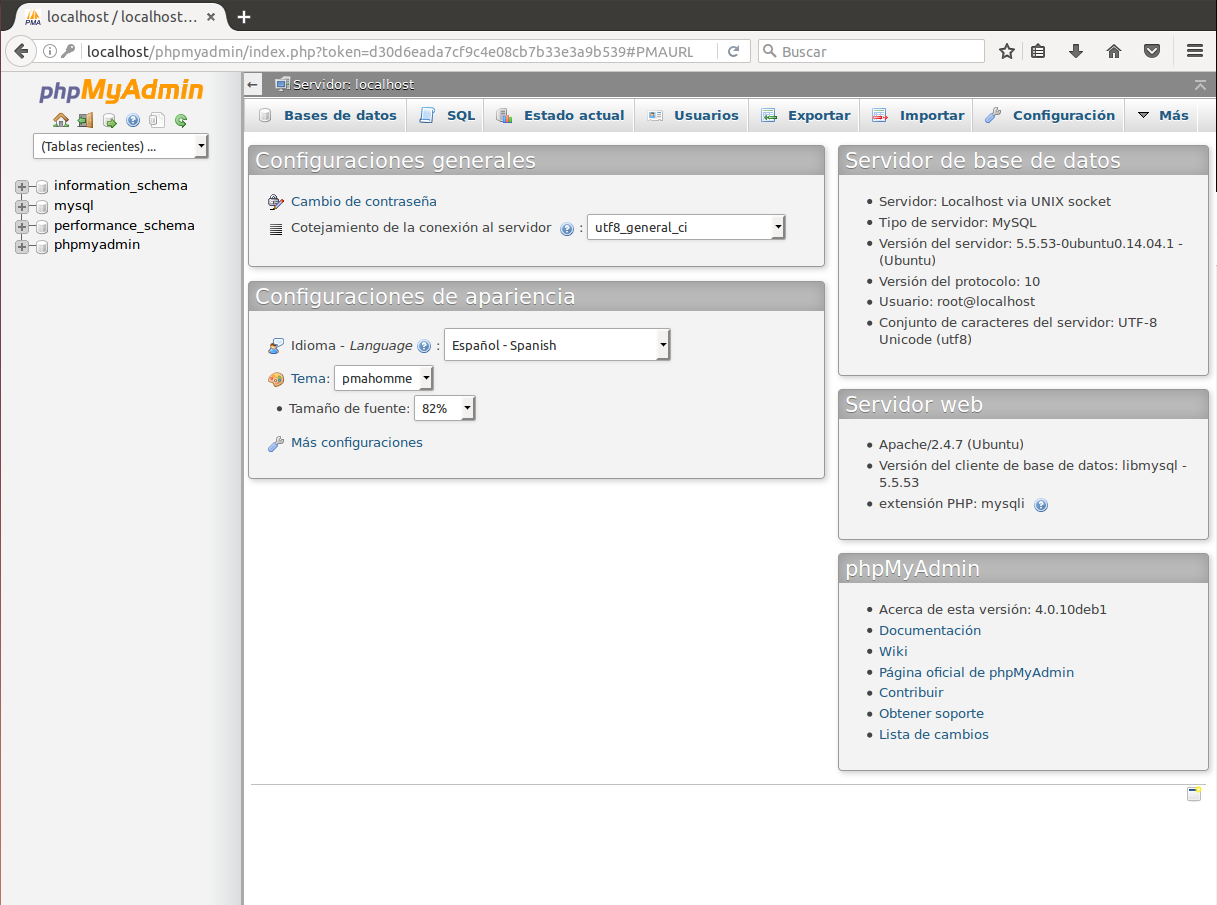
\includegraphics[scale=0.3]{phpmyadmin-localhost}
	\caption{Pantalla de inicio del servicio PHPMyAdmin. - Adrián Morente Gabaldón [23/11/2016]}
	\label{fig:figura23}
\end{figure}
Para terminar, vamos a cambiar el tamaño máximo de subida permitido por el sistema hasta 25MiB. Para ello, accederemos al fichero de configuración \emph{/etc/php5/apache2/php.ini}, que contiene los parámetros modificables de PHP directamente mostrables en el servidor de Apache. Lo podemos abrir con nano en la terminal y buscar \emph{post\_max\_size}, lo que nos mostrará el siguiente fragmento del archivo. Si leemos el texto descriptivo, nos confirma que esta variable define el tamaño máximo aceptado por PHP; pudiendo fijarse a 0 si quisiéramos no establecer ningún límite. Tras la impresión, lo cambiamos a 25MiB.
\begin{figure}[H]
	\centering
	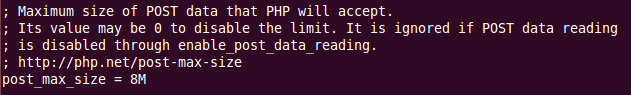
\includegraphics[scale=0.75]{php-max}
	\caption{Configuración del límite de tamaño de bases de datos en PHPMyAdmin. - Adrián Morente Gabaldón [22/11/2016]}
	\label{fig:figura19}
\end{figure}


\section{Visite al menos una de las webs de los software mencionados y pruebe las demos que ofrecen realizando capturas de pantalla y comentando qué está realizando.}
Para esta prueba, veremos el administrador ISPConfig. Si entramos en su página web nos encontramos con unas demostraciones que ofrecen bastante completas \cite{ispconfig}. Si miramos la barra de menú, nos encontramos con varias pestañas, cada una de las cuales nos permite gestionar una parte del servidor: podemos añadir clientes, traductores DNS, dominios de correo electrónico, cambiar datos como contraseña y lenguaje, etc.:
\begin{figure}[H]
	\centering
	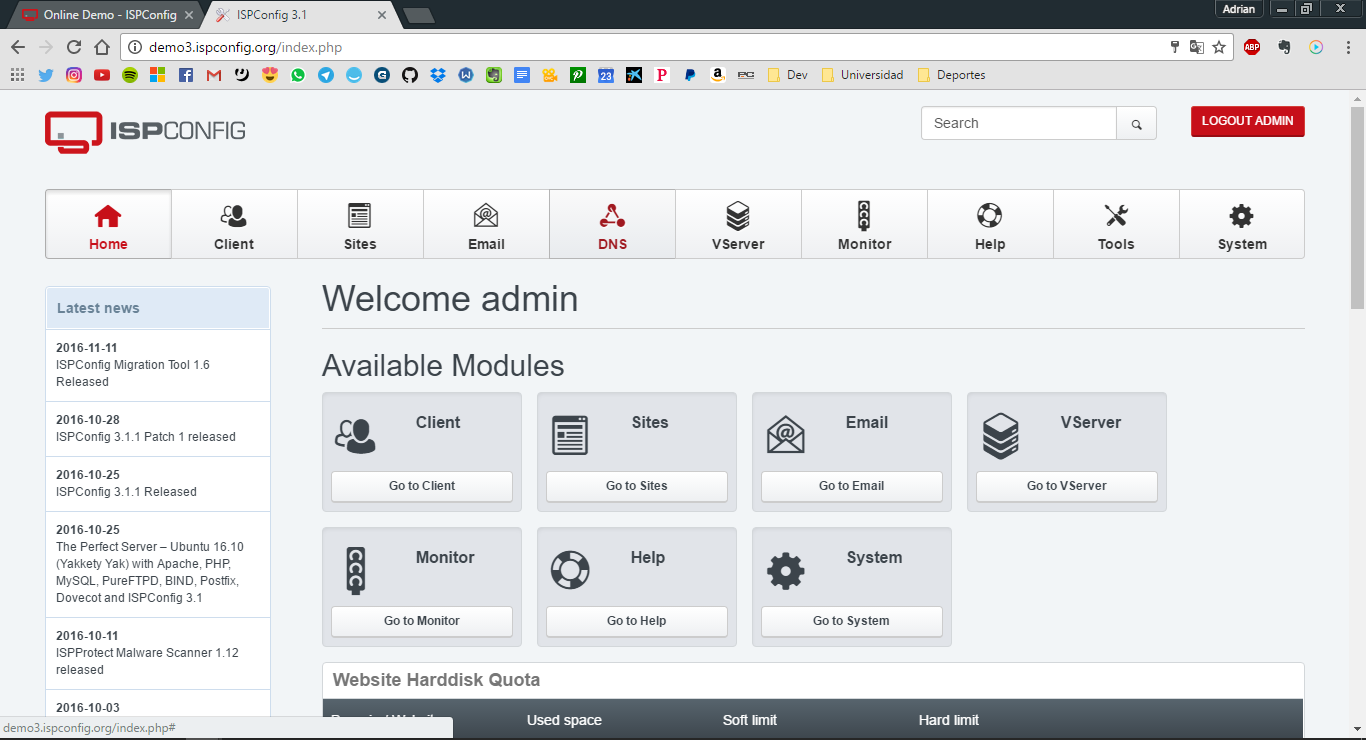
\includegraphics[scale=0.4]{ispconfig-admin}
	\caption{Página de inicio de prueba de ISPConfig. - Adrián Morente Gabaldón [22/11/2016]}
	\label{fig:figura11}
\end{figure}
Para probar una de las funcionalidades ofrecidas, vamos a ver cómo monitorizaríamos uno de los servidores administrados. En la pestaña Monitor encontramos la lista de servidores administrados y el periodo con el que queremos refrescar las estadísticas del profiler usado. En este caso solo tendremos un servidor de prueba ya que, como sabemos, se trata de una demostración gratuita de un servicio de pago. Sin embargo, es ilustrativo en cuanto a las opciones que podemos usar; si miramos el margen izquierdo, encontramos las opciones de monitorización de procesador, CPU, estado de una configuración de discos en RAID, etc. En este caso no podremos cambiar nada por la naturaleza ficticia de la página.
\begin{figure}[H]
	\centering
	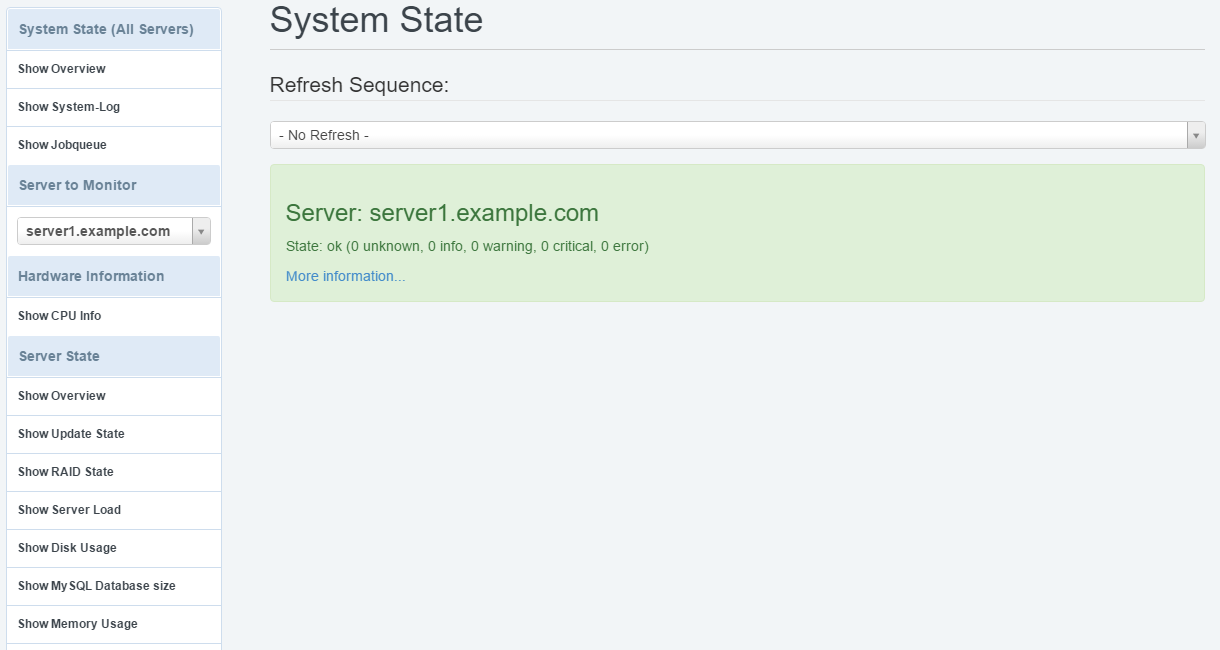
\includegraphics[scale=0.3]{ispconfig-server}
	\caption{Opciones de monitorización de ISPConfig. - Adrián Morente Gabaldón [22/11/2016]}
	\label{fig:figura12}
\end{figure}

\section{a) Ejecute los ejemplos de find, grep b) Escriba el script que haga uso de sed para cambiar la configuración de SSH y reiniciar el servicio. c) Muestre un ejemplo de uso para awk.}

	\subsection{Ejemplos de find y grep}
	El comando grep se utiliza para filtrar cadenas, como bien explica el documento de la práctica. En este caso, hemos ejecutado el ejemplo varias veces, una primera con tres instancias del programa Firefox corriendo, y otra más una vez cerradas. El comando \emph{ps} nos muestra todos los procesos que hay en ejecución en el sistema, que gracias a \emph{grep} filtramos fácilmente. Así nos quedamos con el usuario que está ejecutando el proceso, la hora y el tiempo de ejecución, el directorio y el nombre del proceso, entre otras cosas. Pasemos a ver la captura:
	\begin{figure}[H]
		\centering
		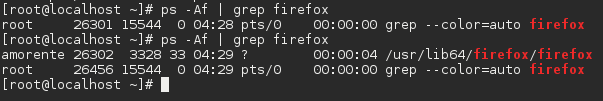
\includegraphics[scale=0.8]{ps-grep}
		\caption{Ejecución de grep filtrando el proceso \emph{firefox}. - Adrián Morente Gabaldón [23/11/2016]}
		\label{fig:figura13}
	\end{figure}

	Por otro lado tenemos el comando find, que lo utilizamos para buscar archivos por el sistema y realizar las acciones que queramos sobre ellos. En cuanto al ejemplo propuesto por la práctica, empezamos listando el contenido de nuestro directorio /home y de las carpetas involucradas (/docs y /PDFs). A continuación, ejecutamos el comando de prueba y vemos como \emph{find} busca los archivos que cumplen el requisito (en este caso, que su nombre termine en \emph{pdf}) y emprende con ellos la acción determinada: copiarlos a la carpeta /PDFs. Una vez hecho, listamos el contenido de esta carpeta para demostrar su efectividad y sencillez de uso.
	\begin{figure}[H]
		\centering
		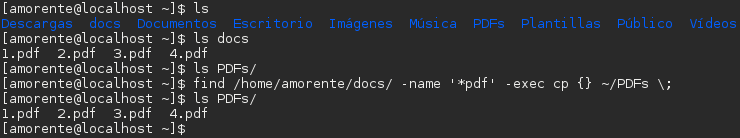
\includegraphics[scale=0.75]{find}
		\caption{Ejecución de find moviendo ficheros entre directorios. - Adrián Morente Gabaldón [23/11/2016]}
		\label{fig:figura14}
	\end{figure}
	
	\subsection{Script de sed para modificar SSH}
	El comando sed nos ayudará a sustituir caracteres o palabras completas por los argumentos que le introduzcamos. Como siempre que modificamos un archivo importante de configuración, es conveniente realizar una copia de seguridad de dicho archivo a uno igual de la forma \emph{archivo.bak}. Pasemos a ver el código implementado en el script para comentarlo:
	\begin{lstlisting}[language=bash]
	#!/bin/bash
	cd /etc/ssh
	puerto\_nuevo = $1
	if[ $puerto\_nuevo -gt 1024 ]; then
	  sed -i "s/22/$puerto_nuevo/1" sshd_config
	  systemctl restart sshd.service
	else
	  echo 'El puerto no puede ser menor de 1024'
	fi
	\end{lstlisting}
	Para empezar, definimos como \$1 el argumento que recibiremos en ejecución, el cual contendrá el número de puerto que pretendemos asignar a la configuración de SSH. Este, como sabemos, deberá ser superior al valor de 1024, ya que los puertos por debajo de este número están reservados.
	Si el número introducido cumple este requisito, llamamos a la herramienta \emph{sed} con los siguientes parámetros:
	\begin{itemize}
		\item \textbf{s}: le pedimos a \emph{sed} que sustituya las dos cadenas especificadas a continuación.
		\item \textbf{22}: el número del puerto que queremos modificar por \$1.
		\item \textbf{\$puerto\_nuevo}: el número introducido como parámetro al programa (\$1).
		\item \textbf{1}: le pedimos que sustituya el primer elemento que encuentra.
		\item \textbf{sshd\_config}: el archivo de entrada al que queremos realizar la modificación.
	\end{itemize}
	A continuación, vemos un ejemplo de la ejecución. Para empezar, imprimos el contenido del archivo de configuración para ver su contenido (puerto 22). A continuación, vemos una ejecución del script errónea, ya que intentamos acceder a un puerto reservado. Justo después, le ponemos un puerto correcto y volvemos a imprimirlo para demostrar su funcionamiento.
	\begin{figure}[H]
		\centering
		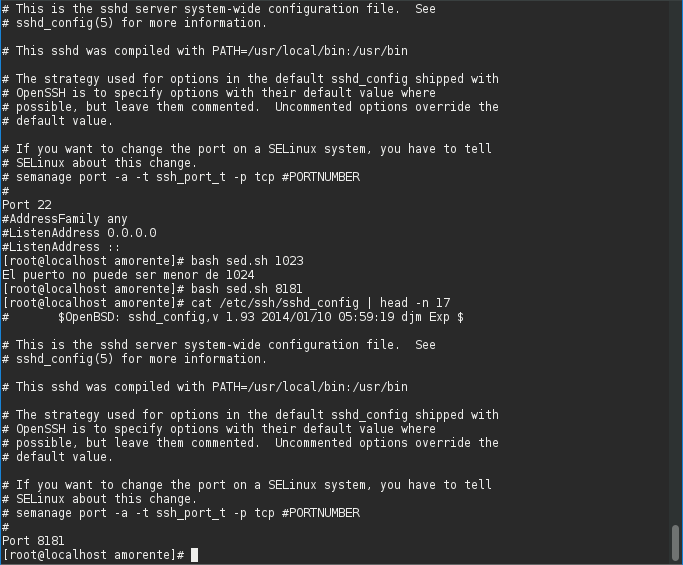
\includegraphics[scale=0.55]{sed-sh}
		\caption{Configuración de SSH a través de la ejecución de un script de sed. - Adrián Morente Gabaldón [24/11/2016]}
		\label{fig:figura16}
	\end{figure}
	
	\subsection{Ejemplo de uso de awk}
	Awk se trata de un lenguaje de programación de procesado de ficheros a muy bajo nivel. Con él podemos programar la manipulación del texto interno de un fichero, como puede ser el de configuración de un servicio, como lo vamos a usar nosotros hoy. Con unas pequeñas líneas de código, podemos conseguir extraer un pequeño fragmento de un archivo, filtrando su contenido. Aunque es de complejidad muy sencilla, nos da una idea de para qué podemos usar esta herramienta. A modo de ejemplo comentaremos el script siguiente:
	\begin{lstlisting}[language=bash]
	awk '/^Port/ { print $2 }' /etc/ssh/sshd_config
	\end{lstlisting}
	Con esta línea estamos diciendo a \emph{awk} que busque la palabra -Port- en aquellas líneas en las que no tenga nada precediéndola. Sabemos que en dicho fichero, tras esa palabra aparece el número de puerto para SSH; que será lo que imprimamos en \$2, que se traduce por la segunda palabra de esa línea. Al final, cerrando el corchete de \emph{awk}, ponemos el archivo en el que queremos buscar. La ejecución de este mini-programa imprime el puerto 22, ya que como sabemos, es el definido por defecto para el servicio SSH.
	\begin{figure}[H]
		\centering
		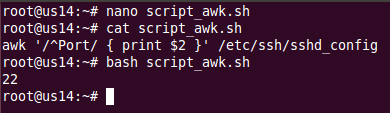
\includegraphics[scale=0.75]{awk}
		\caption{Búsqueda de parámetro de configuración de SSH con la ejecución de un script de awk. - Adrián Morente Gabaldón [24/11/2016]}
	\end{figure}


\section{Escriba el script para cambiar el acceso a SSH usando PHP o Python.}
Para poder modificar el puerto de acceso al servicio SSH, vamos a utilizar un código en Python que se encargue de tomar un parámetro entero mayor de 1024 (ya que como sabemos, los puertos por debajo de dicho valor están protegidos) y sustituirlo en el archivo de configuración. El script consta del siguiente código:
\begin{lstlisting}[language=python]
	import sys
	import fileinput
	
	archivo="/etc/ssh/sshd_config"
	puerto_a_configurar="Port 22"
	arg=sys.argv[1:]
	
	puerto_nuevo="Port "+"".join(arg)
	
	for linea in fileinput.input(archivo, inplace=1):
	  if puerto_a_configurar in linea:
	  linea=linea.replace(puerto_a_configurar, puerto_nuevo)
	  sys.stdout.write(linea)
\end{lstlisting}
Para empezar, definimos la ruta del archivo a configurar, además del puerto configurado inicialmente. A continuación, unimos a la cadena \emph{-Port -} el número de puerto introducido por parámetro. Acto seguido, con la función \emph{replace} de Python sustituimos fácilmente el contenido mencionado del fichero. Justo después, habremos de reiniciar el servicio para que el cambio realizado surta efecto. \\
Veamos la ejecución del programa propuesto. Empezamos imprimiendo una parte del fichero de configuración para comprobar que su puerto está intacto (22). Acto seguido, ejecutamos el script descrito y volvemos a imprimir dicha información, verificando que la modificación se hizo correctamente. Para finalizar, reiniciamos el servicio para que se apliquen los cambios.
\begin{figure}[H]
	\centering
	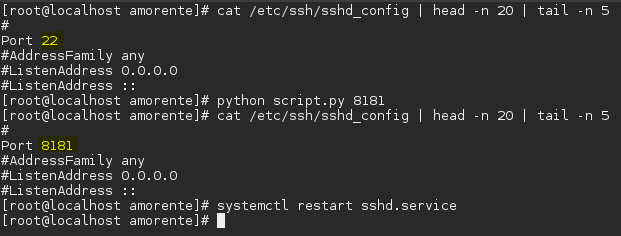
\includegraphics[scale=0.75]{ssh-python}
	\caption{Configuración del puerto de acceso a SSH a través de un script en Python. - Adrián Morente Gabaldón [24/11/2016]}
	\label{fig:figura20}
\end{figure}


\section{Abra una consola de Powershell y pruebe a parar un programa en ejecución, realice capturas de pantalla y comente lo que muestra.}
Aunque la utilización de la consola de Windows para administrar el sistema es mucho más limitada y pesada, también podemos naturalmente comprobar qué procesos se están ejecutando en todo momento en nuestra máquina, y detenerlos si fuera necesario. Para detener un proceso en ejecución podemos hacerlo de dos formas, como bien informa el documento de la práctica:
\begin{itemize}
	\item \textbf{Stop-Process -Name <nombre>}: con este comando detendremos un servicio a partir de su nombre. Esta ha sido la opción que he elegido para la muestra práctica que veremos después.
	\item \textbf{Stop-Process -ID <identificador>}: con este comando detenemos un servicio a partir de su identificador de proceso. Con estos datos ya hemos trabajado en asignaturas como Sistemas Operativos, así que sabemos que cada uno de estos datos identifica unívocamente a un proceso como si de su nombre se tratase. Dicho identificador podemos consultarlo con la orden \emph{Get-Process}, que imprime todos los procesos en curso con sus correspondientes UIDs.
\end{itemize}
Pasemos a ver la ejecución práctica, la cual es extremadamente sencilla. Empezamos obteniendo la lista de procesos con el comando \emph{Get-Process}, y elegimos (por ejemplo) el proceso VBoxTray, el cual se encarga de mantener el icono de las \emph{VirtualBox Guest Additions} a mano en la barra de tareas de Windows. Con el comando mencionado arriba, fácilmente detenemos dicha aplicación. Volvemos a imprimir los procesos en curso para demostrar su detención.
\begin{figure}[H]
	\centering
	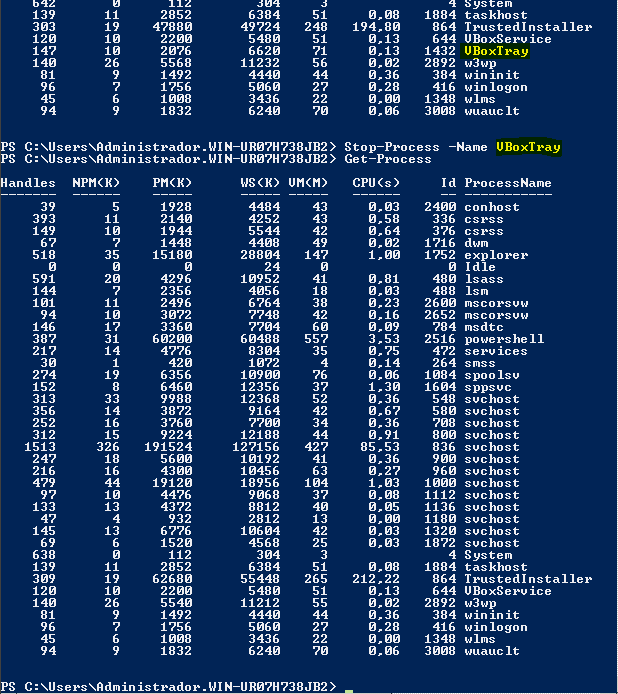
\includegraphics[scale=0.6]{powershell-stop}
	\caption{Detención de un proceso en Windows Server 2008R2 mediante PowerShell. - Adrián Morente Gabaldón [23/11/2016]}
	\label{fig:figura15}
\end{figure}



\bibliography{citas}
\bibliographystyle{plain}
\end{document}
